\documentclass[a4paper,10pt]{report}

\usepackage[utf8]{inputenc}
\usepackage{makecell}
\usepackage{floatrow}
\usepackage{caption}
\floatsetup[table]{capposition=top}
\usepackage{float}
\usepackage{tabularx}
\usepackage{ulem}
\usepackage{graphicx}

\title{Práctica de Búsqueda Local de Inteligencia Artificial}
\author{Josep Maria Olivé Fernández,
        Pol Monroig,
        Yaiza Cano}
\date{20 de marzo del 2020}

\begin{document}

	\maketitle
	
	\section*{Introducción}

    Este proyecto está enfocado principalmente a aprender a resolver un problema mediante algoritmos de búsqueda local explicados en teoría.\newline
    En primer lugar, debemos aprender a razonar sobre la naturaleza del problema y determinar el planteamiento a seguir. Para conseguir esto, se nos ha proporcionado una librería de algoritmos \textit{AIMA} y una que recoge un conjunto de clases que generan los escenarios simulados \textit{DistribFileSystem} que utilizaremos para construir parte de la inicialización nuestro programa.\newline\newline
    Toda la práctica se ha desarrollado en Java, cada experimento se ha realizado 1000 veces y se han calculado valores medios para conseguir resultados más fiables. Los parámetros principales que se han medido a lo largo de la experimentación han sido:
    \begin{itemize}
        \item El tiempo total que se tarda en hallar la solución.
        \item El tiempo que tarda el servidor más lento en gestionar sus peticiones.
        \item El tiempo total de transmisión.
        \item El balance de carga de los servidores.
    \end{itemize}
    Para ilustrar los resultados, se ha hecho uso de gráficas y tablas para complementar las conclusiones y razonamientos extraídos durante la realización de este trabajo.\newline\newline
    Por último, comentar que este proyecto ha sido realizado gracias a la colaboración y el trabajo duro de tres personas.\\\\
    
    \newpage
    \section*{Descripción del Problema}
    
        Muchas aplicaciones en internet necesitan tolerancia a fallos y alta disponibilidad. Una solución frecuente para este problema es el tener un sistema de ficheros distribuido a lo largo de varios servidores y tener otro grupo de servidores dedicados a redireccionar las peticiones de ficheros a los servidores que tienen la copia del fichero pedido.\newline\newline
        El punto clave de esta solución es cómo el servidor que atiende a las peticiones decide qué servidores van a enviar su copia del fichero a su destinatario. Así pues, el objetivo de esta práctica es experimentar con algoritmos de búsqueda local para resolver la tarea de, dado un conjunto de peticiones de ficheros, decidir qué servidores van a responder a dicha petición.\newline\newline
        Una vez encontrada una solución, ¿cómo sabemos si ésta es suficientemente buena? Para evaluar la solución usaremos dos criterios a lo largo de la experimentación que se deberán de optimizar en caso de querer lograr una solución mejor; dichos criterios son:
        \begin{enumerate}
            \item \textbf{Minimizar el tiempo de transmisión} de los ficheros para el servidor que necesita más tiempo para trasmitir sus peticiones.
            \item \textbf{Minimizar el tiempo total de trasmisión} de los ficheros pero con la \textbf{restricción} de que los tiempos de transmisión de los servidores han de ser lo más similares posibles entre ellos.
        \end{enumerate}
        
    \section*{Definición de tipos }
    
        \subsection*{Implementación del estado}
            El estado que representa las soluciones tiene que almacenar de alguna manera las peticiones que hacen los usuarios, es decir tiene que guardar la relación entre petición, servidor e usuario. 
            Al principio pensamos muchas maneras distintas de hacerlo pero muchas tenían inconvenientes, no por que guardaran menos información ni porque no representaran el estado de manera correcta si no porque no eran ineficientes. Lo primero que almacenamos de manera compartida es la información sobre los servidores, esta no representa el estado pero es necesaria para poder cambiar de estado. Después almacenamos una estructura de datos representada por un vector en el cual cada posición del vector representa un fichero y por posición hemos guardado un conjunto de peticiones. Este conjunto de peticiones lo hemos representado con un \textit{MaxHeap} ya que preveíamos su utilidad para poder aplicar los operadores lo mas rápido posible. Por ultimo guardamos otras cualidades sobre el estado para poder calcular los heurísticos mas rápidamente, como por ejemplo un vector donde cada posición de este tenga el sumatorio de tiempos de transición del servidor de esa posición.\clearpage
    
        \subsection*{Tipos de estados iniciales}
            \begin{itemize}
                \item \textbf{initalState1:} Este estado inicial mueve cada petición al servidor que tarda menos en enviarla, escoge el servidor de entre los posibles que pueden enviar ese fichero a dicho usuario. Hemos implementado esta solución inicial ya que hemos pensado que si por cada fichero lo ponemos en un servidor que ya va muy rápido, entonces estamos ayudando al algoritmo a encontrar un estado muy bueno inicialmente. Aunque equilibremos la carga entre servidores. 
                 \item \textbf{initialState2:} Este estado mueve cada petición a un servidor aleatorio de entre los posibles que pueden enviar ese fichero. Hemos elegido esta implementación de solución inicial ya que pensamos basarnos un poco en Simulated Annealing que es estocástico. Al escoger el estado inicial de manera aleatorio estamos provocando una exploración inicial que no esta presente en ningún momento en el Hill Climbing, ya que es un algoritmo que explota y escoge los mejores estados siempre, en otras palabras es puramente greedy. Con esta exploración inicial no estamos seguros de que si obtendremos mejores resultados al o empeoraremos, pero dado que la exploración es mínima lo mas probable es que acabemos obteniendo peores resultados que con el\textit{initialState1}.
            \end{itemize}
        
        \subsection*{Tipos de operadores}
            \begin{itemize}
                \item \textbf{moveMaxFile:} Este operador selecciona el fichero que más tarda del servidor que tiene su suma de tiempos de transmisión más alta y lo mueve a cualquiera de los otros servidores posibles, de manera que tiene un \textit{branch factor} de $k - 1$ donde $k$ es el numero de servidores que contienen dicho fichero. Hemos escogido este heurístico porque creemos que al mover un fichero del servidor mas lento, estamos equilibrando la carga entre servidores. 
            \end{itemize}
            \begin{itemize}
                \item \textbf{moveRandomFile:} Este operador selecciona el fichero que más tarda de un servidor aleatorio y lo mueve a otro servidor aleatorio de los servidores posibles. Tiene el mismo \textit{branch factor} que el operador anterior y lo hemos escogido para ver las diferencias entre un operador fijo y uno aleatorio.
            \end{itemize}
            \begin{itemize}
                \item \textbf{op3:} Este operador combina los primeros dos operadores de la siguiente forma: moveMaxFile $\cup$ moveRandomFile. Tiene un \textit{branch factor} de O(2($k-1$)) donde $k$ es el número de servidores que contienen el fichero que se mueve. Lo hemos escogido para estudiar el comportamiento de la combinación de dos operadores distintos.
            \end{itemize}
            \begin{itemize}
                \item \textbf{op4:} Este operador combina los primeros dos de la siguiente forma: moveMaxFile $\cap$ moveRandomFile. Tiene un \textbf{brach factor} de O($k-1$) donde $k$ es el número de servidores que contiene el fichero que se mueve. Lo hemos escogido en contrapunto al operador anterior.
            \end{itemize}
            
        \subsection*{Tipos de heurístico}
            \begin{itemize}
                \item \textbf{FirstHeuristicFunction:} Este heurístico tiene en cuenta el sumatorio de tres criterios 
                    \begin{equation}
                        h(state) = h_1(state) + h_2(state) + h_3(state) 
                    \end{equation}
                    donde $h_1$ es el el tiempo del servidor que tarda mas, $h_2$ es el total de todos los tiempos de transmisión 
                    y $h_3$ es el equilibrio de tiempos de transmisión entre servidores y esta representada por la varianza. 
                \item \textbf{SlowestServerHeuristicFunction} Este heurístico representa el criterio $h_1$.
                \item \textbf{TwoHeuristicFunction} Este heurístico representa 
                el criterio $h_1$ + el criterio $h_2$.
            \end{itemize}
        
        \subsection*{Tipos de generadores de sucesores}
            \begin{itemize}
                \item \textbf{FirstSuccessorFunction:} Genera todos los sucesores de un estado aplicando el operador \textit{moveMaxFile}.
                \item \textbf{SecondSuccessorFunction:} Genera todos los sucesores de un estado aplicando el operador \textit{moveRandomFile}.
                \item \textbf{ThirdSuccessorFunction:} Genera todos los sucesores de un estado aplicando el operador {op3}, que es una combinación entre {moveMaxFile} y {moveRandomFile}.
            \end{itemize}
        
        
        
    \newpage
	\section*{Experimento 1}
	
		En este experimento, nuestro objetivo es descubrir qué combinación de nuestros \uline{operadores} es el más efectivo, es decir, con el que obtenemos mejores resultados a partir de una misma inicialización. El criterio que determinará la resolución de la prueba es el de minimizar el tiempo de transmisión del servidor que más tarda en gestionar sus peticiones.
		
		\subsection*{Hipótesis}
		\textbf{"El operador \textit{moveMaxFile}, comparado con los otros operadores bajo las mismas condiciones, será el que obtenga el menor tiempo de transmisión del servidor más lento"}.

		\subsection*{Condiciones iniciales del experimento}
		\begin{itemize}
		    \item Nº de usuarios: 200.
    		\item Nº máximo de peticiones por usuarios: 5.
    		\item Nº servidores: 50.
    		\item Nº mínimo de replicaciones: 5.
    		\item Algoritmo: Hill Climbing.
    		\item Estrategia de inicialización: initialState2.
    		\item Heurístico usado: SlowestServerHeuristicFunction.
    		\item Operadores usados: Todos, ya que son el sujeto de la prueba. 
		\end{itemize}
		
		\subsection*{Resultados del experimento}
		\begin{table}[H]
		\centering
        \begin{tabular}{c|c|c}
            Operadores & Situación inicial & Situación final \\
            \hline
            \hline
            moveMaxFile & 56.883 & 39.864 \\
            \hline
            moveRandomFile & 56.883 & 56.876\\
            \hline
            \makecell{moveMaxFile $\cup$ \\moveRandomFile} & 56.883 & 39.863 \\
            \hline
            \makecell{moveMaxFile $\cap$ \\moveRandomFile} & 56.883 & 56.833 
        \end{tabular}
        \caption*{Fichero que más tarda: \textit{MaxTransmissionTime}}
        \end{table}
        
	\subsection*{Conclusiones}
	Analizando los resultados obtenidos vemos que nuestra hipótesis era errónea. En un principio pensamos que con el primer operador obtendríamos los mismos resultados que con el tercero pero en menor tiempo y, por lo tanto, sería mejor.\\
	Lo que nos llevo a creer esto es que el tercer operador no es más que lo que obtenemos del primero más la unión de un seguido de estados sucesores generados de manera aleatoria por el segundo operador; así que pensamos que estos últimos estados no tendrían relevancia ya que el primer operador está programado con el objetivo de obtener lo que nosotros considerábamos los mejores estados sucesores posibles.\\
	De todas formas, decidimos llevar este experimento un paso más allá aun que no se pedía: al ver que la diferencia entre resultados del op1 con el op3, decidimos valorar también el tiempo que tardaban cada uno en encontrar solución y los resultados obtenidos son los siguientes: 22ms vs 43ms. El op3 tarda el doble que el op1, así que hemos decidido quedarnos con este último.\\
	De este experimento hemos aprendido a no subestimar la aleatoriedad y que añadir un poco de ellas a nuestras fórmulas no está de más. Además, para hacer un buen trabajo, a veces hay que seguir el criterio de aquellos que lo realizan y no solo de los establecidos matemáticamente.
	
	
	
	\newpage
	\section*{Experimento 2}

		El objetivo de este segundo experimento es averiguar qué estrategia de \uline{estado inicial} da mejores resultados y fijar, de esta manera, el mejor estado sobre el que se partirá en la realización de los siguientes experimentos. El criterio que determinará la resolución de la prueba es el mismo que el del experimento anterior.
		
	    \subsection*{Hipótesis}
		\textbf{"El estado \textit{initialState1}, comparado con el otro estado bajo las mismas condiciones, será el que obtenga el menor tiempo de transmisión del servidor más lento"}.
	
		\subsection*{Condiciones iniciales del experimento}
		\begin{itemize}
		    \item Nº de usuarios: 200.
    		\item Nº máximo de peticiones por usuarios: 5.
    		\item Nº servidores: 50.
    		\item Nº mínimo de replicaciones: 5.
    		\item Algoritmo: Hill Climbing
    		\item Estrategia de inicialización: Todas, son el sujeto de la prueba. 
    		\item Heurístico usado: SlowestServerHeuristicFunction.
    		\item Operador usado: op1.
		\end{itemize}

		\subsection*{Resultados del experimento}
		\begin{table}[H]
		\centering
        \begin{tabular}{c|c|c}
            Estados & Situación inicial & Situación Final \\
            \hline
            \hline
            initialState1 & 19.022 & 14.709 \\
            \hline
            initialState2 & 56.883 & 39.864 \\
        \end{tabular}
        \caption*{Fichero que más tarda: MaxTransmissionTime}
        \end{table}
        
        \subsection*{Conclusiones}
        Analizando los resultados obtenidos podemos comprobar la certeza de nuestra hipótesis.\\
        En este experimento teníamos bastante claro que el primer estado daría mejores resultados que el segundo pero tampoco nos imaginábamos que la diferencia sería tan grande.\\ 
        Como complemento a la reflexión de los resultados del experimento anterior vemos que aunque un poco de aleatoriedad esté bien, mucha puede ser contraproducente. Nuestro segundo estado tiene un factor de aleatoriedad muy grande y hace que sea difícil encauzarlo a una solución que se pueda considerar suficientemente buena.\\
        También nos gustaría comentar que nos ha sorprendido que el operador y el heurístico hayan reducido tanto el tiempo, pensábamos que al partir de un estado inicial tan malo, no serían tan eficaces pero han conseguido reducirlo en un 29.9\% vs el 22.7\% del primer estado.\\
        De este experimento hemos interiorizado el concepto de que la eficacia del operador y del heurístico no dependen del estado al que se le aplique pero que tampoco pueden hacer magia. 
        
        
        
	\newpage
	\section*{Experimento 3}

		Una vez tenemos la mejor estrategia de inicialización y la mejor combinación de operadores, aplicamos el mismo heurístico y definimos las mismas condiciones de prueba pero cambiando el algoritmo inteligente. El algoritmo a usar es \textit{Simulated Annealing} y el objetivo de este experimento es averiguar con qué \uline{parámetros} da mejores resultados. El criterio que determinará la resolución de la prueba será el mismo que hemos estado utilizando hasta ahora. \\\\
		El planteamiento de este experimento es un poco caótico, hemos decidido que la mejor manera de obtener resultados es incrementando el valor de uno de los parámetros en cada ejecución mientras mantenemos fijado el de los otros tres.\\
		
		Los parámetros son los siguientes:\\
		
		\begin{tabular}{c|c}
		\centering
		    Parámetros & Significado \\
		    \hline
		    \hline
		    steps & número de temperaturas. \\
		    \hline
		    stiter & número de iteraciones dentro de cada temperatura. \\
		    \hline
		    k & valor temperatura inicial. \\ 
		    \hline
		    lamb & decremento de temperatura. \\
		\end{tabular}\\\\
		
		Sus valores son estos:
		\begin{itemize}
		    \item Para \textit{steps} variable partiendo de un valor de 250 e incrementándolo 250 en cada ejecución hasta un límite de 2000:

		    \begin{itemize}
		        \item stiter: 50.
		        \item k: 50.
		        \item lamb: 0.005.
		    \end{itemize}
		    \item Para \textit{stiter} variable partiendo de un valor de 25 e incrementándolo 25 en cada ejecución hasta un límite de 300:
		    \begin{itemize}
		        \item steps: 500.
		        \item k: 50.
		        \item lamb: 0.005.
		    \end{itemize}
		    \item Para \textit{k} variable partiendo de un valor de 25 e incrementándolo 25 en cada ejecución hasta un límite de 300:
		    \begin{itemize}
		        \item steps: 500.
		        \item stiter: 50.
		        \item lamb: 0.005.
		    \end{itemize}
		    \item Para \textit{lamb} variable partiendo de un valor
		    \begin{itemize}
		        \item steps: 500.
		        \item stiter: 50.
		        \item k: 225.
		    \end{itemize}
		\end{itemize}
		
		
		\subsection*{Hipótesis}
		\textbf{"Los valores que dan mejor resultado en el algoritmo inteligente \textit{Simulated Anneling} son: \textit{steps} = 1000", \textit{stiter} = 150, \textit{k} = 50 i \textit{lambda} = 0.005."}
		
		\subsection*{Condiciones iniciales del experimento}
		\begin{itemize}
		    \item Nº de usuarios: 200.
    		\item Nº máximo de peticiones por usuarios: 5.
    		\item Nº servidores: 50.
    		\item Nº mínimo de replicaciones: 5.
    		\item Algoritmo: Simulated Annealing.
    		\item Parámetros del algoritmo: sujetos de la prueba. 
    		\item Estrategia de inicialización: initialState1.
    		\item Heurístico usado: SlowestServerHeuristicFunction.
    		\item Operador usado: op1.
		\end{itemize}

		\subsection*{Resultados del experimento}
		
		\begin{figure}[H]
        \minipage{0.5\textwidth}
          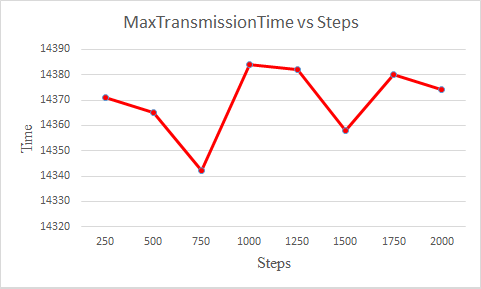
\includegraphics[width=\linewidth]{images/Time vs Steps.png}
        \endminipage\hfill
        \minipage{0.5\textwidth}%
          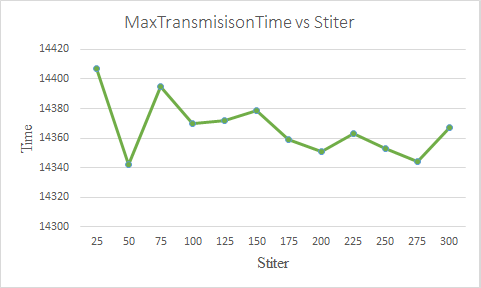
\includegraphics[width=\linewidth]{images/Time vs Stiter.png}
        \endminipage
        \end{figure}
        
        \begin{figure}[H]
        \minipage{0.5\textwidth}
          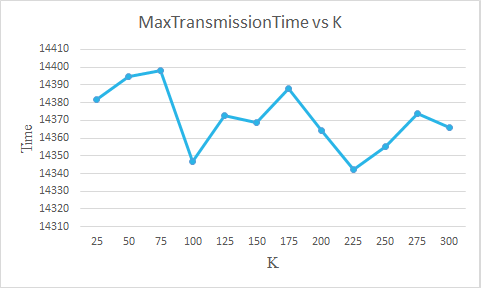
\includegraphics[width=\linewidth]{images/Time vs K.png}
        \endminipage\hfill
        \minipage{0.5\textwidth}%
          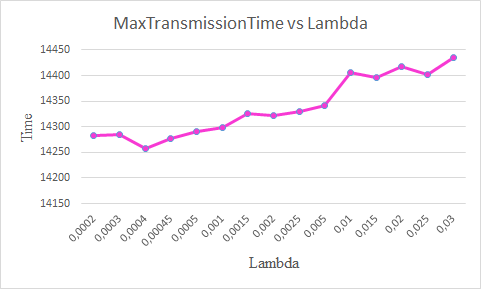
\includegraphics[width=\linewidth]{images/Time vs Lambda.png}
        \endminipage
        \end{figure}
        
        \subsection*{Conclusiones}
        La primera conclusión clara que podemos extraer de este experimento es que nuestra hipótesis inicial era totalmente errónea, y que el valor óptimo para \textit{steps} es de 750, y no de 1000. Mientras que el valor óptimo para el \textit{Stiter} es 50, para la \textit{K} es 225 y para \textit{Lambda} 0,004.
		
		
		
	\newpage
	\section*{Experimento 4}

		Esta vez queremos estudiar la evolución del \uline{tiempo de ejecución} del algoritmo \textit{Hill Climbing} según el número de usuarios y el número de servidores. Al tener dos parámetros distintos a evaluar, lo que haremos es fijar uno de ellos e ir incrementando el otro hasta que se pueda datar su tendencia y luego viceversa. \\
		Primero fijaremos el número de servidores en 50 y los usuarios los iremos incrementando de 100 en 100 partiendo de un valor de 100. Una vez encontrada la tendencia, fijaremos el número de usuarios en 200 e incrementaremos los servidores de 50 en 50, partiendo de un valor de 50.\\
		El criterio que determinará la resolución de la prueba será el mismo que hemos estado utilizando hasta ahora.
		
		\subsection*{Hipótesis}
		\textbf{"A menor numero de servidores, mayor sera el rendimiento."}
		
		\subsection*{Condiciones iniciales del experimento}
		\begin{itemize}
		    \item Nº de usuarios: variable.
    		\item Nº máximo de peticiones por usuarios: 5, constante.
    		\item Nº servidores: variable.
    		\item Nº mínimo de replicaciones: 5, contante.
    		\item Algoritmo: Hill climbing.
    		\item Estrategia de inicialización: initialState1.
    		\item Heurístico usado: SlowestServerHeuristicFunction.
    		\item Operador usado: op1.
		\end{itemize}

		\subsection*{Resultados del experimento}
		
		\begin{figure}[H]
        \minipage{0.5\textwidth}
          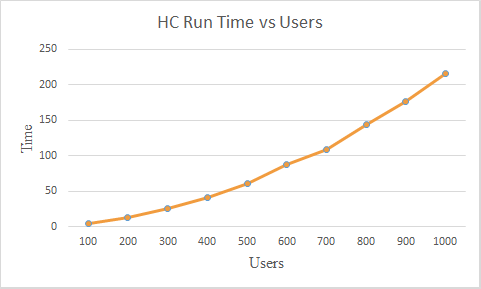
\includegraphics[width=\linewidth]{images/Run Time vs Users.png}
        \endminipage\hfill
        \minipage{0.5\textwidth}%
          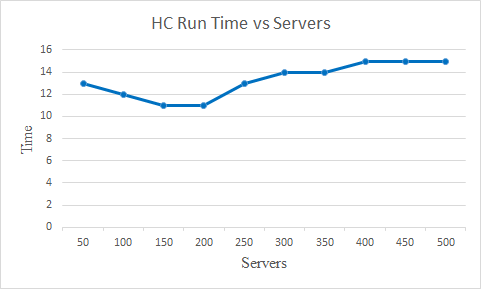
\includegraphics[width=\linewidth]{images/Run Time vs Servers.png}
        \endminipage
        \end{figure}
		
		\subsection*{Conclusiones}
		Vemos que lo que afecta realmente al rendimiento no es tanto el numero de servidores, sino el numero de replicaciones mínimo que hay que mantener, ya que es este numero el que nos va a marcar el coste de nuestros operadores. Juntamente con el numero de usuarios que debemos gestionar.
		
		
	\newpage
	\section*{Experimento 5}
        
		En este caso se ha implementado un nuevo heurístico que tenga en cuenta dos criterios distintos, y a partir de esto se calcula la diferencia entre el tiempo total de transmisión y el tiempo para hallar la solución, las condiciones son las mismas que las del primer apartado.\newline

        \subsection*{Hipótesis}
		\textbf{"Creemos que este nuevo heurístico dará un resultado final mejor que un heurístico que solo tenga en cuenta un solo criterio."}

		\subsection*{Condiciones iniciales del experimento}
		\begin{itemize}
		    \item Nº de usuarios: 200.
    		\item Nº máximo de peticiones por usuarios: 5.
    		\item Nº servidores: 50.
    		\item Nº mínimo de replicaciones: 5.
    		\item Algoritmo: Hill Climbing.
    		\item Estrategia de inicialización: initialState1.
    		\item Heuristico usado: FirstHeuristicFunction y SlowServerHeuristicFunction.
    		\item Operador usado: op1.
		\end{itemize}

		\subsection*{Resultados del experimento}
		\begin{table}[H]
		\centering
        \begin{tabular}{c|c|c}
            Time & First & Slow \\
            \hline
            \hline
            Elapsed & 6 & 13 \\
            \hline
            Total Transmisión & 515.636 & 562.434 \\
        \end{tabular}
        \end{table}
        
		
		\subsection*{Conclusión}
		Vemos finalmente que el heurístico FirstHeuristicFunction que tiene en cuenta dos criterios más que el SlowServerHeuristicFunction da resultados mucho mejores, pues esta mucho más quilificado para ver si un estado es de mayor o menor calidad. A demás vemos también que el tiempo empleado por este heurístico es menor, y por lo tanto también es más eficiente. Aun así, SlowServerHeuristicFunction es mejor si solo deseamos reducir el tiempo mínimo, ya que al solo fijarse en este factor, realiza mejor esta tarea en concreto.
		
		
	\newpage
	\section*{Experimento 6}

		Consiste en repetir el experimento anterior cambiando el algoritmo inteligente a \textit{Simulated Annealing}.

        \subsection*{Hipótesis}
		\textbf{"Visto el resultado anterior, suponemos que FirstHeuristicFunction nos dará mejores resultados."}

		\subsection*{Condiciones iniciales del experimento}
		\begin{itemize}
		    \item Nº de usuarios: 200
    		\item Nº máximo de peticiones por usuarios: 5
    		\item Nº servidores: 50
    		\item Nº mínimo de replicaciones: 5
    		\item Algoritmo: SimulatedAnnealing
    		\item Parámetros del algoritmo: 
    		\begin{itemize}
    		    \item steps = 750.
    		    \item stiter = 50.
    		    \item k = 225.
    		    \item lambda = 0.004.
    		\end{itemize}
    		\item Estrategia de inicialización: initialState1
    		\item Heuristico usado: FirstHeuristicFunction y
    		SlowServerHeuristicFunction.
    		\item Operador usado: op1.
		\end{itemize}

		\subsection*{Resultados del experimento}
		\begin{table}[H]
		\centering
        \begin{tabular}{c|c|c}
            Time & First & Slow \\
            \hline
            \hline
            Elapsed & 193 & 195 \\
            \hline
            Total Transmisión & 507.456 & 609.689 \\
        \end{tabular}
        \end{table}
		
		\subsection*{Conclusión}
		Vemos otra vez que FirstHeuristicFunction nos da un tiempo de transmisión final mejor que SlowServerHeuristicFunction, y que a demás, el tiempo que necesita para darnos la solución es muy ligeramente menor, por lo tanto seria arriesgado decir que FirstHeuristicFunction es más eficiente en este caso, pero aun así es innegable que el resultado de este es mejor.
		
		
	\newpage
	\section*{Experimento 7}

		Este experimento consiste en medir el \uline{tiempo total de transmisión} y el \uline{tiempo necesario para hallar la solución} para diferentes valores de número de replicaciones de un fichero.\newline
		Usando el escenario inicial decidido en el \textit{Experimento 2}, el algoritmo \textit{Hill Climbing} y ambas heurísticas, iremos incrementando el valor de número de replicaciones de 5 en 5, partiendo desde 5 y llegando a un límite de 25. 
		
		\subsection*{Hipótesis}
		\textbf{"Basándonos en resultados anteriores, creemos que a menor numero de replicaciones mayor será nuestro tiempo de ejecución."}

		\subsection*{Condiciones iniciales del experimento}
		\begin{itemize}
		    \item Nº de usuarios: 200.
    		\item Nº máximo de peticiones por usuarios: 5.
    		\item Nº servidores: 50.
    		\item Nº mínimo de replicaciones: variable, son el sujeto de la prueba.
    		\item Algoritmo: Hill Climbing.
    		\item Estrategia de inicialización: initialState1
    		\item Heuristico usado: FirstHeuristicFunction.
    		\item Operador usado: op1.
		\end{itemize}

		\subsection*{Resultados del experimento}
		
		\begin{figure}[H]
        \minipage{0.5\textwidth}
          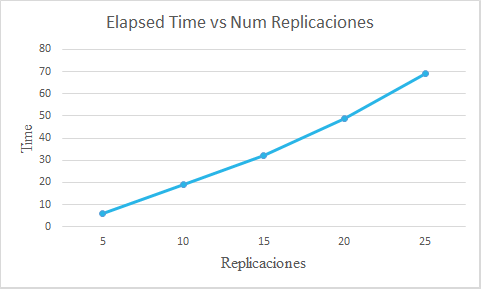
\includegraphics[width=\linewidth]{images/Elapsed Time vs Num Replicaciones.png}
        \endminipage\hfill
        \minipage{0.5\textwidth}%
          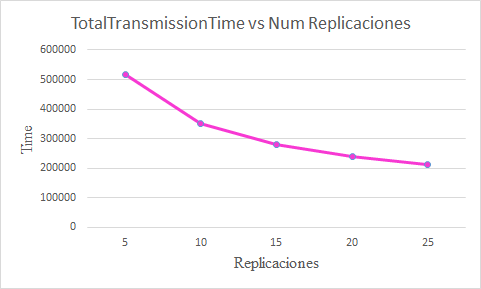
\includegraphics[width=\linewidth]{images/TotalTime vs Num Replicaciones.png}
        \endminipage
        \end{figure}
		
		\subsection*{Conclusión}
		Vemos que nuestra hipótesis era correcta, y que a menor numero de replicas, menor es el coste de nuestros operadores y por lo tanto menor tiempo de ejecución tenemos. Por otro lado, a mayor numero de replicas, menor puede llegar a ser nuestro tiempo de transmisión total, ya que tendremos la posibilidad de usar un mayor numero de servidores para el mismo fichero, facilitándonos reducir la carga individual de cada uno, y encontrando un mayor numero de rutas óptimas o sub-óptimas.
		
	\newpage
	\section*{Conclusión del proyecto}
    A lo largo de este trabajo hemos tenido nuestra primera toma de contacto con el mundo de inteligencia artificial y hemos podido ver fácilmente la cantidad de posibilidades que ofrece la librería \textit{AIMA} y lo útil que nos podrá ser cuando hagamos algún proyecto que se pueda resolver utilizando algoritmos de \textit{búsqueda local}, técnica de resolución de problemas explicada en clase de teoría y que hemos logrado comprender después de invertir horas a esta práctica.\newline
    Además, en este proyecto hemos aprendido cómo diseñar experimentos, recopilar datos, extraer resultados, analizarlos y sacar conclusiones. También hemos aprendido a trabajar en equipo y la importancia del uso de herramientas colaborativas como \textit{git} y \textit{Overleaf}.\newline\newline
	Como bonus, nos gustaría comentar que nos hemos dado cuenta de la importancia de pasar todos los juegos de pruebas posibles para cerciorarse de que el output proporcionado es aceptable. Si no hubiera sido porque decidimos invertir tiempo necesario para realizar el experimento especial y obtener feedback antes de la fecha de entrega de la práctica, no nos hubiéramos dado cuenta de un error en la implementación y no hubiéramos sido capaces de entender los resultados obtenidos durante la parte de experimentación.	        


	
\newpage
\begin{flushleft}
\textbf{INFORMACIÓN DEL TRABAJO DE INNOVACIÓN} \\
\end{flushleft}
    Para nuestro trabajo de innovación hemos decidido realizar un estudio sobre \textit{AlphaStar}, la primera IA que ha sido capaz de derrotar a uno de los mejores jugadores profesionales de \textit{StarCraft II}, un videojuego de estratégia creado por \textit{Blizzard Entertainment}.\\\\
    Dicho trabajo aún está en proceso y lo hemos divido en las siguientes secciones:
    \begin{enumerate}
        \item Introducción: terminada y hecha por \textbf{Yaiza Cano}.
        \item Descripción del producto: terminada y hecha por \textbf{Yaiza Cano}.
        \item Métodos y técnicas utilizadas: en proceso y hecho por \textbf{Pol Monroig}.
        \item Factor innovador del producto: terminado y hecho por \textbf{Josep Maria Olivé}.
    	\item Impacto del producto en la empresa: en proceso.
    	\item Impacto del producto en el usuario o en la sociedad: en proceso.\\
    \end{enumerate}
    Para documentar, hicimos uso de la siguiente lista de referencias:
    \begin{itemize}
        \item \uline{Reinforcement learning:} libro utilizado para los apartados \textbf{Métodos y técnicas utilizadas i Factor innovador del producto}.
        \item \uline{AlphaStar Grandmaster level in StarCraft II using multi-agent reinforcement learning:} artículo en el blog \textit{Deepmind} utilizado para los apartados \textbf{Descripción del producto, Métodos y técnicas utilizadas i Factor innovador del producto}.
        \item \uline{AlphaStar Grandmaster level in StarCraft II using multi-agent reinforcement learning:} paper en la revista \textit{Nature} utilizado para los apartados \textbf{Descripción del producto, Métodos y técnicas utilizadas i Factor innovador del producto}.
        \item \uline{Artificial intelligence in video games:} artículo en \textit{Wikipedia} utilizado para el apartado \textbf{Introducción}.
        \item \uline{AlphaStar: Mastering the Real-Time Strategy Game StarCraft II:} artículo en el blog \textit{Deepmind} utilizado para los apartados \textbf{Métodos y técnicas utilizadas, Factor innovador del producto}.
        \item \uline{Play nim game:} juego en \textit{Archimedes-lab} utilizado para el apartado \textbf{Factor innovador del producto}.
        
    \end{itemize}
    El hecho de que \textit{StarCraft II} sea conocido por su dificultad, además de ser uno de los juegos más famosos (por no decir el más) y con más visualizaciones en los \textit{E-Sports}, ha hecho que sea realmente complicado encontrar información útil o suficientemente técnica que podamos aprovechar ya que, aunque la creación revolucionaria de la IA \textit{AlphaStar} haya dado lugar a que exista mucha cantidad de información sobre ella y que se hable de ella en muchas páginas web, dicha información está enfocada a su público, un público genérico y no especializado.\\
\end{document}
